\chapter{Proving correctness of \textit{np-convert-assignments}}\label{chap:proof}
While the entire Chez Scheme compiler translates Scheme to machine code, the \caname\ pass performs a single intermediate step in this process by performing a Scheme-to-Scheme transformation on some expressions. As its name suggests, the purpose of the \caname\ pass is to \textit{convert} variable \textit{assignment} expressions to a different form. Since both the source and target languages are Scheme, we can reason about the pass solely using Scheme's formal \textit{operational semantics}, a rigorously defined standard for reducing Scheme expressions.

We will first review the pass itself and the transformation that it performs. Then, we will define our notion of semantic preservation, and use some properties of the semantics as well as some relations defined atop it to show that the transformation does indeed preserve the semantics of a program.
\section{The \textit{np-convert-assignments} pass\label{sxn:ca-pass}}
\subsection{Assumptions}
One important note about \caname\ is that it uses special, decorated expressions in both its source and target languages. Since we do not have have a formal framework for asserting the meaning of these decorated Chez Scheme expressions, we make the critical assumption that they abide to the relevant rules of the R6RS formal semantics. From observation, this assumption seems to hold true, as the decorated expressions can be consistently \textit{erased} down to normal Scheme expressions (see Figure \ref{fig:chez_erase} for an example of a term in the source language of \caname\ compared to its \textit{erased} version in the language defined by the formal semantics).

\begin{figure}[h]
    \centering
    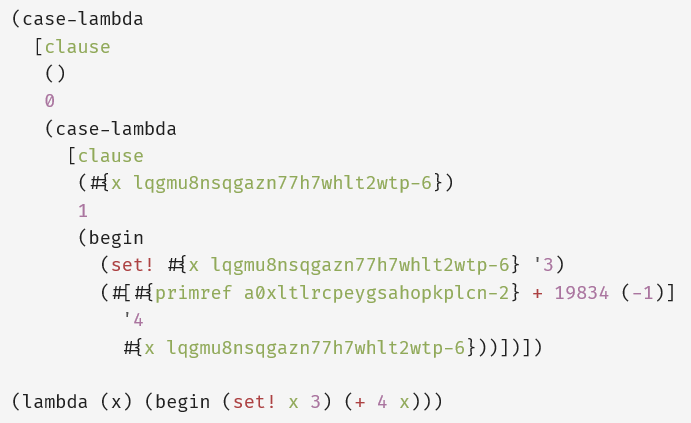
\includegraphics[scale=0.75, keepaspectratio]{figures/chez_erase.png}
    \caption{Example of \textit{erasing} Chez Scheme term decoration.}
    \label{fig:chez_erase}
\end{figure}

Another area where we must make an assumption is in developing a model of \caname\ to reason about. The code for actually executing the pass contains and operates on expressions that are not covered by the R6RS semantic model. Therefore, we attempt to faithfully recreate the effects of the transformation on the expressions in subset of the formal semantics that we are considering. Our analogous \caname\ function was created through careful examination of the source code and observation of input and output of the pass for various examples.

\subsection{Intuition}
The \textit{np-convert-assignments} pass removes indefinite-extent assignments and replaces them with assignments that have a defined scope. This pass is quite small, defined in about 40 lines in the production Chez Scheme compiler. The size of our proof and accompanying frameworks relative to the size of the transformation is a testament to the difficulty of verifying compilation correctness.

The intuition for the pass is best acquired through observing a few examples:

\begin{figure}[h]
    \centering
    \begin{enumerate}
        \item $ca_{e}$(set! x v) = (set-car! $x^{*}$ $\hat{v}$)
        \item $ca_{e}$(lambda (x) (set! x v)) = \newline (lambda (t) ((lambda (x) (set-car! x $\hat{v}$))(cons t null))) \newline \textit{Where t is fresh}
        \item $ca_{prog}$(store ((x $v$)) x) = (store (($pp_x$ (cons $\hat{v}$ null))) (car $pp_x$))
    \end{enumerate}
    Where $\hat{A}$ means the appropriate $ca$ function applied to A.
    
    $x^{*}$ could either be $x$ or $pp_x$ depending on the context.
    \caption{Motivating examples of the \caname \ pass.}
    \label{fig:ca_examples}
\end{figure}

The first example shows the primary action of the pass --- to remove set! expressions. Depending on if x is in the store or enclosed in a lambda, we may transform it into a pointer or not, as shown in the next two examples. Notice the recursive call to $ca_e$ on $v$.

The second example shows how lambda expressions are modified to support the transformation of set! expressions. Since its arguments are now assumed to be cons cells, we have to first wrap its arguments inside of a list. Also note that we do not change the $x$ to $pp_x$, as at this point it is just a representation of the lambda's argument.

Finally, the last example shows how $ca$ deals with partially evaluated programs. Since the \textbf{appN!} rule is the only one that can create new non-list store locations, we can assume that variables in the store correspond to previously evaluated lambda abstractions. Therefore, we must treat variables and set! expressions that refer to store locations as transformation targets. We also retroactively convert these previously evaluated store locations. In this case, we do change $x$ to $pp_x$, so that expressions that contain it can properly evaluate.

% Some explanation for these examples is required. The first example is one of the simplest --- it transforms a variable reference to a call to \textit{car} on a pair pointer representing that variable. We will see in the next examples why this pair pointer conversion is necessary, but we can see clearly the transformation that occurs to variable references. It is also important to note a slight abuse of our notation in this example: that we perform transformation on an evaluation context ($\hat{P}$). While the pass does not actually operate on decomposed programs, we use this notation for clarity and to be able to isolate transformations on specific parts of a program. In section \ref{sxn:ctx_trans}, we show that this way of transforming a program that is decomposed into a context and an expression is the same as transforming the program before decomposition.

% The second example shows the main purpose of the transformation --- to remove indefinite extent set! expressions from the language and replace them with set-car!. One important note about $x$ in this example is that it is always referring to a bound variable, though the lambda expression that bound it may have already been evaluated, as we consider in example 4. In that case, we know the variable was bound because it will be present in the store. Because we are not allowing top-level variables in our subset of the semantics, we can make this assumption and transform all set! that we encounter.

% The third example demonstrates the transformation of a lambda expression that contains an assigning set! expression. The original lambda expression is wrapped in an additional lambda expression and applied to the argument of that lambda expression wrapped in a cons cell. We can also see the transformation of the assigning set! expression. The purpose of this specific transformation is to make sure that all of the set! calls and variable references inside the lambda expression still work. Since they have been transformed to operate on lists, this step of the transformation ensures that they will always receive a list as their argument.

% The fourth example exhibits the behavior of the transformation on a partially evaluated program. Since the \textbf{appN!} semantic rule is the only rule that adds variables to the store, we can assume that if a variable is in the store, it was the target of a set! somewhere in the body of the lambda that was evaluated using \textbf{appN!} (since this is a side condition of the rule). Therefore, for the transformation to work correctly on partially evaluated programs, we need to transform each variable in the store that is not already a pair pointer. Note that all variables transformed this way are converted to pair pointers, since they now refer to cons cells. Therefore, after a transformation, our store will contain only pair pointers.

\subsection{Definition}
We now formally define our model of the transformation as the following functions on the syntax of our language:

\begin{definition} {\large\textbf{ca$_{prog}$}} --- Programs

$ca_{prog}(store\ (sf \dots)\ e) = (store\ (ca_{sf}(sf) \dots)\ ca_e(e)) $

\end{definition}

\begin{definition} {\large\textbf{ca$_{sf}$}} --- Store Locations

$ca_{sf}(x\ v) = (pp_x\ (cons\ v\ null))$

$ca_{sf}(pp\ (cons\ v\ null)) = (pp\ (cons\ v\ null))$
\end{definition}

\begin{definition} {\large\textbf{ca$_e$}} --- Expressions

$ca_e(begin\ e\ e\ \dots) = (begin\ ca_e(e)\ ca_e(e)\ \dots)$

$ca_e(e\ e\ \dots) = (ca_e(e)\ ca_e(e)\ \dots)$

$ca_e(set!\ x\ e) = (set \mhyphen car!\ pp_x\ ca_e(e))$

\qquad where x is in the store.

$ca_e(set!\ x\ e) = (set \mhyphen car!\ x\ ca_e(e))$

\qquad where x is not in the store.

$ca_e(values\ v) = (values\ ca_e(v))$

$ca_e(x) = (car\ pp_x)$

\qquad where x is in the store.

$ca_e(x) = (car\ x)$

\qquad where x is not in the store.

$ca_e(lambda\ (x)\ e) = (lambda\ (t)\ ((lambda\ (x)\ ca_e(e))(cons\ t\ null)))$

\qquad where x is the target of a set! in e, t is fresh.

$ca_e(lambda\ (x)\ e) = (lambda\ (x)\ ca_e(e))$ 

\qquad where x is not the target of a set! in e.

All other expressions are unchanged by $ca_e$.

\end{definition}

Finally, we define $ca_{ctx}$ for use in applying the pass to decomposed programs.

\begin{definition} {\large\textbf{ca$_{ctx}$}} --- Evaluation Contexts

$ca_{ctx}(store\ (sf\ \dots)\ F^{*}) = (store\ (ca_{sf}(sf)\ \dots)\ ca_{ctx}(F^{*}))$

$ca_{ctx}(v\ \dots\ F^{\circ}\ v\ \dots) = (ca_e(v)\ \dots\ ca_{ctx}(F^{\circ})\ ca_e(v)\ \dots)$

$ca_{ctx}(if\ F^{\circ}\ e\ e) = (if\ ca_{ctx}(F^{\circ})\ ca_e(e)\ ca_e(e))$

$ca_{ctx}(set!\ x\ F^{\circ}) = (set \mhyphen car!\ pp_x\ ca_{ctx}(F^{\circ}))$

\qquad where x is in the store.

$ca_{ctx}(set!\ x\ F^{\circ}) = (set \mhyphen car!\ x\ ca_{ctx}(F^{\circ}))$

\qquad wher x is not in the store.

$ca_{ctx}(begin\ F^{*}\ e\ e\ \dots) = (begin\ ca_{ctx}(F^{*})\ ca_e(e)\ ca_e(e)\ \dots)$

$ca_{ctx}([\ ]) = ca_{ctx}([\ ]^{*}) = ca_{ctx}([\ ]^{\circ}) = [\ ]$

\end{definition}

\subsection{Lemmas}
Here we prove some properties of the \caname\ functions that are necessary for our later proofs.

\begin{lemma}\label{lem:trans_val} Transformation Preserves Values

If v is a value, then $ca_e(v)$ is a value.
\end{lemma}
\begin{proof}
By induction on the structure of our values.

For most values, $ca_e$ makes no changes. For these cases, $ca_e(v)$ is trivially a value.

The only value expression which is modified by $ca_e$ is $(lambda\ (x)\ e)$, where x is the target of a set! inside of e. We can observe the transformation:

$ca_e((lambda\ (x)\ e)) = (lambda\ (t)\ ((lambda\ (x)\ ca_e(e))(cons\ t\ null)))$

We can clearly see that this is still a value, since it is of the form $(lambda\ (t)\ e')$, where $e' = ((lambda\ (x)\ ca_e(e))(cons\ t\ null))$

Therefore, we have shown that $ca_e$ preserves the value status of values that it transforms.
\end{proof}

\begin{lemma}\label{lem:trans_expr} Transformation Preserves Expressions

If e is a non-value expression, then $ca_e(e)$ is a non-value expression.
\end{lemma}
\begin{proof}
The non-value expressions that get transformed by $ca_e$ are:

\begin{enumerate}
    \item $x$
    \item $(set!\ x\ v)$
\end{enumerate}

$ca_e(x)$ evaluates to either $(car\ x)$ or $(car\ pp_x)$, both of which are still expressions.

$(set!\ x\ v)$ similarly evaluates to either $(set \mhyphen car!\ x\ \hat{v})$ or $(set \mhyphen car!\ pp_x\ \hat{v})$, which are again both still expressions.

Therefore, if $e$ is a non-value expression, $ca_e(e)$ will always be a non-value expression.

\end{proof}

\begin{lemma}\label{lem:trans_decomp} Transformation Preserves Decomposition

$ca_{prog}(C[p]) = ca_{ctx}(C)[ca_e(p)]$

for all evaluation contexts C and expressions p.

\end{lemma}
\begin{proof} We proceed by induction on the structure of our evaluation contexts.

Consider the cases of C: $(store (sf ...) F^{*})$

and the cases of $F^{*}$: $[\ ]^{*}$, $F$.

If $F^{*}$ is a hole, then we must show that 

$ca_{prog}((store (sf ...)\ p)) = ca_{ctx}((store (sf ...) [(ca_{e}(p))]))$

which follows from the definitions of $ca_{prog}$ and $ca_{ctx}$.

Otherwise, consider the cases of F: $[\ ]$, $(v \dots F^{\circ}\ v \dots)$, $(if\ F^{\circ}\ e\ e)$, $(set!\ x\ F^{\circ})$, and $(begin\ F^{*}\ e\ e \dots)$.

$[\ ]$ follows by definitions as before. 

In the case of  $(v \dots F^{\circ}\ v \dots)$, $(if\ F^{\circ}\ e\ e)$, $(begin\ F^{*}\ e\ e \dots)$, $ca_{ctx}$ makes no structural changes to the context other than the expected calls to $ca_{ctx}$ and $ca_e$ on sub-expressions. Therefore, it follows from our induction principle and the definitions of $ca_{ctx}$, $ca_e$ that the transformation preserves decomposition in these cases.

The interesting case, $(set!\ x\ F')$, has a transformation occur in the evaluation context. There are two possibilities for the transformation of $(set!\ x\ F')$:

\begin{enumerate}
    \item $ca_{ctx}(set!\ x\ F') = (set \mhyphen car!\ pp_x\ ca_{ctx}(F'))$ if x is in the enclosing store.
    \item $ca_{ctx}(set!\ x\ F') = (set \mhyphen car!\ x\ ca_{ctx}(F'))$ if x is not in the store (i.e. if x is bound by a lambda expression in some enclosing context).
\end{enumerate}

In case 1, we need to show that:

$ca_{prog}(store\ (sf \dots)\ (set!\ x\ F'[p])) = ca_{ctx}(store\ (sf \dots)\ (set!\ x\ ca_{ctx}(F')[ca_e(p)])$

Since we know x must be in the store, 

$ca_{prog}(store\ (sf \dots)\ (set!\ x\ F'[p])) = (store\ (ca_{sf}(sf) \dots) (set \mhyphen car!\ pp_x\ ca_{e}(F'[p])))$. 

This case follows by definition of $ca_{e}$ and $ca_{ctx}$, and by our induction principle.

Case 2 follows similarly, except that x is not in the store, so 

$ca_{prog}(store\ (sf \dots)\ (set!\ x\ F'[p])) = (store\ (ca_{sf}(sf) \dots) (set \mhyphen car!\ x\ ca_{e}(F'[p])))$. 

Therefore, we have shown that our transformation preserves decomposition for all cases.
\end{proof}








\newpage
\section{Proof Overview}
To prove that $ca_{prog}$ preserves the semantics of programs that it transforms, we must consider what we mean by semantic preservation. Since $ca_{prog}$ entirely removes an expression, set!, we cannot expect the transformed program to take \textit{exactly} the same steps. It seems reasonable, then, to say that a program's semantics are preserved over a transformation if the transformed program takes \textit{equivalent} steps. 

To formalize this informal definition, we must first define a way for a program to take multiple steps:
\begin{definition}
Transitive, reflexive closure of $\step$
\begin{enumerate}
    \item $a$ \trstep\ $c$ if $a$ \trstep\ $b$ and $b$ \trstep\ $c$ (Transitivity)
    \item $a$ \trstep\ $a$ (Reflexivity)
    \item $a$ \trstep\ $b$ if $a \step\ b$ (Closure)
\end{enumerate}
\end{definition}

The intuition for the reflexive, transitive closure of $\step$ is that it relates expressions that have zero or more single steps between them.

Our definition of step \textit{equivalence} uses the idea of simulation. That is, if a relation is a simulation relation, then related programs take equivalent semantic steps. The intuition for such a relation is shown by Figure \ref{fig:sim_diagram}. We formally define our notion of a simulation relation in section \ref{sxn:sim}.

\begin{figure}
    \centering
    \begin{tikzpicture}[label/.style = {  }]
  \tikzset{every node/.style={anchor=center, text centered}} 
  \matrix (m)
    [
      matrix of math nodes,
      row sep    = 5em,
      column sep = 7em
    ]
    {
      P & P' & \dots & P'' & \\
      ca_{prog}(P) & ca_{prog}(P') & \dots & ca_{prog}(P'') \\
    };
  \foreach \i in {1, 2} {
    \path
      let \n1 = { int(\i+1) } in
        [line width=0.5mm ] (m-1-\i) edge [|->] node [above, label] {} (m-1-\n1)
        [line width=0.5mm ]  (m-2-\i) edge [|->>] node [below, label] {} (m-2-\n1);
  }
  \foreach \i in {1,...,3} {
    \path
      let \n1 = { int(\i+1) } in
          [line width=0.5mm] (m-1-\i) edge [dashed] node [left,  label] {} (m-2-\i);
  }
  \path [line width=0.5mm]  (m-1-3) edge [|->] node [left,  label] {} (m-1-4)
        [line width=0.5mm] (m-2-3) edge [|->>] node [left,  label] {} (m-2-4)
        [line width=0.5mm] (m-1-4) edge [dashed] node [left, label] {} (m-2-4);
\end{tikzpicture}
    \caption{Simulation relation visualization}
    \label{fig:sim_diagram}
\end{figure}

If we can show that $ca_{prog}$ is a simulation, then we know that $P$ and $ca_{prog}(P)$ take equivalent steps and therefore that $ca_{prog}$ preserves the semantics of the programs it transforms.

As a summary, our definitions so far are as follows:
\begin{table}
    \centering
    \begin{tabular}{ |c|p{6cm}|p{6cm}| } 
 \hline
 Symbol & Definition \\ 
 \hline
 $\step$& A single, standard, reduction step defined by the semantics. \\ 
 \trstep & The reflexive, transitive closure of $\step$ \\
 $ca_{prog}$ & $ca$ on programs. \\
 $ca_{ctx}$ & $ca$ on evaluations contexts. \\
 $ca_{sf}$ & $ca$ on store locations. \\
 $ca_{e}$ & $ca$ on expressions. \\ 
 \hline
\end{tabular}
    \caption{Definitions}
    \label{tab:defs}
\end{table}


Our proof is structured as follows:
\begin{enumerate}
    \item Show that our semantics is deterministic (Section \ref{sxn:det_sem}).
    \item Prove that $ca_{prog}$ is a simulation relation (Section \ref{sxn:sim}).
\end{enumerate}


\subsection{Deterministic Semantics}\label{sxn:det_sem}
An implicit assumption made by figure \ref{fig:sim_diagram} is that our programs follow a canonical reduction order. That is, that a program P will always step to the same P'. Another way of stating this is by saying that our semantics are \textit{deterministic}.

\begin{definition} Deterministic Relation

If a relation R is deterministic then,

$\forall a\ b_1\ b_2, a\ R\ b_1, a\ R\ b_2 => b_1 = b_2$.

\end{definition}

In the context of our semantics, we state this theorem as follows:

\begin{theorem}\label{thm:step_det}


\textbf{Single Step Deterministic}

$\forall P\ P_1\ P_2,\ P\ \step\ P_1,\ P\ \step\ P_2\ => P_1 = P_2$


\end{theorem}

To prove Theorem \ref{thm:step_det}, we will first show a property of all programs called the VSR property. This property states that P is either a \textbf{V}alue, \textbf{S}tuck, or \textbf{R}educible. In the context of our semantics, we say that that P is reducible if it can be decomposed into a context C and expression e such that $C[e]\ \step\ C'[e']$ for some $C'[e']$ on the right hand side of a semantic step. To show that our semantics are deterministic, we strengthen this property to require uniqueness of the evaluation context C that P decomposes into.

\begin{lemma}\label{lem:vsr} VSR Property for Programs

$\forall P,$ P is one of the three:
\begin{enumerate}
    \item $P = (store\ (sf\ \dots)\ v)$ --- Value
    \item $\lnot\ \exists P',\ P\ \step P'$ --- Stuck
    \item $\exists\ unique\ C, \ P = C[e], C[e]\ \step\ C'[e']$ --- Reducible
\end{enumerate}
\end{lemma}
\begin{proof} By induction on the structure of our expressions.

The only case of P is $(store\ (sf\ \dots)\ e)$.

We can see that the VSR property holds for a program if it holds for the program's expression:

If $e$ is a value, then $P = (store\ (sf\ \dots)\ v)$.

If $C[e]$ has no applicable semantic steps to take, we say $e$ is stuck. Clearly in this case, $\lnot\ \exists P',\ P=C[e]\ \step P'$

Finally, if $e = F[e']$ such that e' is a reducible expression, then $C[e] = C[F[e']]$ has a valid semantic step. We refer to this as $e$ being \textit{reducible}.

We proceed by induction on $e$.

If $e$ is a value, then we are done.

Otherwise, if e is not a value, consider the cases:

\textbf{Case 1: $e = (begin\ e_1\ e_2\ \dots)$}

We know by induction hypothesis that all $e_i$ in the body of the begin expression are either values, stuck, or reducible.

Consider when $e_2\ \dots$ is empty. Therefore, $e = (begin\ e_1)$. Hence, we can directly apply the \textbf{beginD} rule. Therefore, e is reducible, and the unique context is simply the store and an empty hole.

If $e_2\ \dots$ is not empty, then consider the case where $e_1$ is a value. Then, we can decompose $e$ into $F[v]$, where $F = (begin\ [\ ]^{*}\ e_2\ e_3\ \dots)$. The \textbf{promote} rule is applicable here, and there is no other decomposition we can perform on e. Therefore, this case falls under reducible. Next, consider when $e_1$ is stuck. Similar to the value case, the evaluation context for begin applies to e, but since $e_1$ is not a value, \textbf{promote} is not applicable. Therefore, we are stuck, since there is no applicable rule or further decomposition that would allow a step to be taken. Finally, consider the case where $e_1$ is reducible. Since $e_1$ is not a value, \textbf{promote} again cannot apply.  Then, we can decompose e into $F[e_1']$, where $F = (begin\ [\ ]\ e_2\ e_3\ \dots)$. Since \textbf{promote} and \textbf{beginD} are not applicable, F is the unique decomposition, with whichever reduction step $F[e_1']$ takes being the only applicable step.

\textbf{Case 2: $e = (if\ e_1\ e_2\ e_3)$}

If $e_1$ is a value, then either \textbf{ifT} or \textbf{ifF} are applicable, and $e$ is clearly reducible, with the unique context just being the store and an empty hole.

Otherwise, if $e_1$ is stuck and not a value, then $e$ is stuck. 

Similarly, if $e_1$ is reducible, then $e$ is reducible:

$e = F[e_1]$, where $F = (if\ [\ ]\ e_2\ e_3)$.

\textbf{Case 3: $e = (e_1\ e_2\ \dots)$}

Again, we know that all $e_i$ in the body of e are either values, stuck, or reducible.

Consider when all $e_i$ are values. Then, there can be various rules applied, depending on the specific value of each $e_i$: \textbf{cons, car, cdr, set-car!, set-cdr!, appN!, appN, app0} and all of the arithmetic rules are potentially applicable here. If none of these rules are applicable, then $e$ is stuck, since none of $e_i$ are further reducible.

If all of $e_i$ are stuck, then $e$ can take the \textbf{mark} step and is therefore reducible (though it will be stuck immediately after). The same follows if all of $e_i$ are reducible, except it will continue to take steps after.

Now, consider if $e_i$ are a mix of stuck, reducible, and value expressions. There are three possible cases here:

\begin{enumerate}
    \item $e$ can be decomposed into $F[e_i]$, where $F = (v\ \dots\ F^{\circ}\ v\ \dots)$.
    \item The \textbf{mark} rule is applicable.
    \item $e$ is stuck.
\end{enumerate}

We know this because \textbf{mark} is the only semantic rule applicable to $(e_1\ e_2\ \dots)$ expressions with non-value sub-expressions. However, due to the requirement of \textbf{mark} that $e_2\dots$ contains a non-value expression, it is never the case that \textbf{mark} can be applicable and $e$ can be decomposed using the $(v\ \dots\ F^{\circ}\ v\ \dots)$ evaluation context at the same time.

Therefore, consider the possibilities of $e_1$ in the decomposition case. $e_1$ cannot be a value, since then all of $e_i$ would be values. If $e_1$ is reducible, then that is the semantic step that $e$ must take. Otherwise, if $e_1$ is stuck, then $e$ is stuck, since all other $e_i$ are values.

In the \textbf{mark} and stuck cases, $e$ is clearly reducible and stuck respectively.


\textbf{Case 4: $e = (set!\ x\ e_1)$}

If $x$ is not in the store, e is clearly stuck, so we assume $x$ is in the store.

Again, by induction principle, $e_1$ must be a value, stuck, or reducible.

If $e_1$ is a value, the \textbf{set!} rule is applicable.

Otherwise, if not, $e$ is stuck if $e_1$ is, or reducible if $e_1$ is.

\textbf{Case 5: $e = (values\ v)$}

If $e$ is in a $[\ ]^{\circ}$ context, then \textbf{demote} is applicable, and $e$ is therefore reducible. Otherwise, it is stuck.

\textbf{Case 6: $e = x$}

If $x$ is in the store, then \textbf{var} is applicable, and $e$ is therefore reducible. Otherwise, $e$ is stuck.

By showing this property for all cases of P and e, we have proven it is true for all programs by induction principle.
\end{proof}

Since we have shown that if a program reduces, it does so by decomposing uniquely into an evaluation context and a reducible expression, Theorem \ref{thm:step_det} follows from Lemma \ref{lem:vsr}. 

% In case 2, we again know that all expressions in the body of e have the unique evaluation context decomposition property.

% However, case 2 is quite different from case 1 in that there are several semantic rules that apply to various sequences of values. For this part of the proof, rather than doing case analysis on several $e_i$ values simultaneously, we will instead look closely at applicable semantic rules and the sequence evaluation context to show that sequence expressions decompose uniquely.

% All of the list-oriented semantic rules require that the sequence is entirely filled with values. Therefore, if e = ($v_1$ $v_2$ ...), there are two possibilities: 
% \begin{enumerate}
%     \item There is an applicable semantic rule. In this case, e uniquely decomposes to a hole and itself.
%     \item There is no applicable semantic rule. We can apply the sequence evaluation context, but since e is comprised entirely of values, no step can be taken in any of the decompositions. Therefore, e is stuck.
% \end{enumerate}

% Next, we consider when there are non-value $e_i$ expressions in the body of e. The two remaining semantic rules both only apply in this case. If e is of the form ($e_1$  ...), the only applicable rule is \textit{mark1}. The sequence evaluation context is not applicable because $e_1$ 



% (set! $x$ $t$), where $t$ is some non-value expression, has no corresponding semantic rule. However, this expression can be decomposed into $E[t]$, where $E = $ (set! $x$ []). Since there are no other evaluation contexts for set! expressions, and no semantic rule for set! with a non-value as its second argument, this decomposition is unique.

% The other cases follow similarly to \textit{set!}. Cleverly and necessarily, there are no expressions with directly applicable semantic rules that can also be decomposed into an evaluation context that isn't just an empty hole.

\subsection{$ca_{prog}$ is a simulation relation.\label{sxn:sim}}
In this section we show that the relation defined by the \textit{np-convert-assignments} pass is a simulation relation. First, we formally define our notion of simulation:

\begin{definition} \textbf{Simulation Relation}

If a relation R is a simulation, and $aRb$, then:

$a\ \step\ a' => \exists\ b', b$ \trstep\ $b', a'Rb'$
\end{definition}

That is, if $a$ and $b$ are related by a simulation relation, and $a\ \step\ a'$, then there must exist $b'$ such that $b$ \trstep\ $b'$ and that $a'$ is related to $b'$. Thus, to show that $ca$ is a simulation relation, we must show that if $P\ \step\ P'$, then there exists a ${P^{*}}$ such that $ca_{prog}(P)\ \trstep\ {P^{*}}, ca_{prog}(P') = {P^{*}}$.

Therefore, if we can show that for each possible single semantic step, that transforming the left hand side and then stepping a finite number of times always arrives at the transformation of the right hand side, then we have shown that $ca_{prog}$ is a simulation relation.

One thing to note is that since we are considering the decomposed programs that $\step$ operates on, we make implicit use of Lemma \ref{lem:trans_val} throughout our proof to relate these findings back to $ca_{prog}$.


\begin{theorem}\label{thm:step} \textbf{Step Theorem}


$P\ \step\ P' =>\\ \exists {P^{*}}\ such\ that\\ \ ca_{prog}(P)\ \trstep\ {P^{*}}\ and\\ \qquad ca_{prog}(P') = {P^{*}}$.

\end{theorem}
\begin{proof} By induction on the structure of P.

By Lemma \ref{lem:vsr}, P must be a value, be stuck, or be decomposible into a unique evaluation context C and a  expression e such that one of the semantic rules applies.

If P is a value or stuck, the theorem is trivial by contradiction.

Otherwise, P must be in the form of the left hand side of one of the semantic rules. Our proof follows by case analysis of the semantic rules.

The most interesting example comes from the rule \textbf{appN!}. This should make sense, since \textbf{appN!} corresponds to lambda applications that contain assignments, and $ca_{prog}$ removes all assignments. Indeed, we will confirm from the steps that correspond to \textbf{appN!} that assignments are removed.

First, we define some convenient notation:
\begin{table}[h]
    \centering
    \begin{tabular}{c}
         $\hat{P} = ca_{prog}(P)$  \\
         
        $\hat{C} = ca_{ctx}(C)$     \\

        $\hat{sf} = ca_{sf}(sf)$    \\

        $\hat{e} = ca_e(e)$     \\
    \end{tabular}
    \caption{Notation for various $ca$ functions}
    \label{tab:ca_notation}
\end{table}

Now, consider the semantic step \textbf{appN!}, taking $P$ to $P'$: 
\[
P = (store\ (sf \dots) F[((lambda\ (x)\ e)\ v)])\ \step 
\]
\[
P' = (store\ (sf \dots (p\ v)) F[(lambda\ ()\ \{x \xrightarrow{} p\}\ e)]) \quad (p\ fresh,\ x\ assigned\ to\ in\ e)
\]

$P$ transforms to $\hat{P}$:
\[
\hat{P} = (store\ (\hat{sf} \dots) \hat{F}[((lambda\ (t)\ ((lambda\ (x)\ \hat{e})(cons\ t\ null))\ \hat{v}))]) \quad (t\ fresh)
\]

$P'$ transforms to $\hat{P'}$:
\[
\hat{P'} = (store\ (\hat{sf} \dots (pp\ (cons\ \hat{v}\ null)) \hat{F}[(lambda\ ()\ \{x \xrightarrow{} pp\}\ \hat{e})])
\]

If $ca$ is a simulation, $\hat{P}$ must take a finite amount of steps and arrive at a $P^{*}$ such that $P^{*} = \hat{P'}$.

We propose that $\hat{P}$ will take 5 steps to get to $P^{*}$.
\begin{enumerate}
    \item We first apply the \textbf{appN} rule to $\hat{P}$, since t is fresh.
    \[
    (store\ (\hat{sf} \dots) \hat{F}[((lambda\ (t)\ ((lambda\ (x)\  \hat{e})(cons\ t\ null))\ \hat{v}))])\ \step
    \]
    \[
    (store\ (\hat{sf} \dots) \hat{F}[((lambda\ ()\ ((lambda\ (x)\  \hat{e})(cons\ \hat{v}\ null))))])
    \]
    \item Then, we apply \textbf{app0}.
    \[
    (store\ (\hat{sf} \dots) \hat{F}[((lambda\ ()\ ((lambda\ (x)\  \hat{e})(cons\ \hat{v}\ null))))])\ \step
    \]
    \[
    (store\ (\hat{sf} \dots) \hat{F}[((begin\ ((lambda\ (x)\  \hat{e})(cons\ \hat{v}\ null))))])
    \]
    \item Now, we apply \textbf{beginD}.
    \[
    (store\ (\hat{sf} \dots) \hat{F}[((begin\ ((lambda\ (x)\  \hat{e})(cons\ \hat{v}\ null))))])\ \step
    \]
    \[
    (store\ (\hat{sf} \dots) \hat{F}[((lambda\ (x)\  \hat{e})(cons\ \hat{v}\ null))])
    \]
    \item At this point, to apply the \textbf{cons} rule, we must first decompose our program into an evaluation context and a reducible expression. We do so as follows:
    \[
    (store\ (\hat{sf} \dots) \hat{F}[((lambda\ (x)\  \hat{e})(cons\ \hat{v}\ null))]) = 
    \]
    \[
    (store\ (\hat{sf} \dots) \hat{F^{+}}[(cons\ \hat{v}\ null)])
    \]
    where $\hat{F^{+}} = \hat{F}[((lambda\ (x)\ \hat{e})[\ ])]$.
    
    We can then reduce using the \textbf{cons} rule:
    \[
    (store\ (\hat{sf} \dots) \hat{F^{+}}[(cons\ \hat{v}\ null)])\ \step
    \]
    \[
    (store\ (\hat{sf} \dots (pp\ (cons\ \hat{v}\ null))) \hat{F^{+}}[pp])
    \]
    And expand our context:
    \[
    (store\ (\hat{sf} \dots (pp\ (cons\ \hat{v}\ null))) \hat{F^{+}}[pp]) = 
    \]
    \[
    (store\ (\hat{sf} \dots (pp\ (cons\ \hat{v}\ null)))\hat{F}[((lambda\ (x)\ \hat{e})\ pp)]
    \]
    
    
    \item Finally, we can apply \textbf{appN} again, since pp is fresh.
    \[
    (store\ (\hat{sf} \dots (pp\ (cons\ \hat{v}\ null))) \hat{F}[((lambda\ (x)\  \hat{e})\ pp)])\ \step
    \]
    \[
    (store\ (\hat{sf} \dots (pp\ (cons\ \hat{v}\ null))) \hat{F}[(lambda\ ()\  \{x \xrightarrow{} pp\}\ \hat{e})])
    \]
\end{enumerate}

Comparing this result to $\hat{P'}$, we can see they are the same. Therefore, if $P$ takes step \textbf{appN!}, $\hat{P}$ takes the steps \textbf{appN, app0, beginD, cons, appN} in order to arrive at a $P^{*}$ that satisfies our simulation definition. Figure \ref{fig:appn!_steps} visualizes this relationship.

\begin{figure}[h]
    \centering
    \begin{tikzpicture}[label/.style = {  }]
  \tikzset{every node/.style={anchor=center, text centered}} 
  \matrix (m)
    [
      matrix of math nodes,
      row sep    = 2em,
      column sep = 4em
    ]
    {
      P & & & & & P' \\
      \hat{P} & P^{1} & P^{2} & P^{3} & P^{4} & P^{*} \\
    };
    \path
        (m-2-1) edge [|->] node [above, label] {appN} (m-2-2)
        (m-2-2) edge [|->] node [above, label] {app0} (m-2-3)
        (m-2-3) edge [|->] node [above, label] {beginD} (m-2-4)
        (m-2-4) edge [|->] node [above, label] {cons} (m-2-5)
        (m-2-5) edge [|->] node [above, label] {appN} (m-2-6)
        (m-2-6) edge [dashed] node [] {} (m-1-6)
        (m-1-1) edge [dashed] node [] {} (m-2-1)
        (m-1-1) edge [|->] node [above, label] {appN!} (m-1-6);
\end{tikzpicture}
    \caption{Simulation of \textbf{appN!}}
    \label{fig:appn!_steps}
\end{figure}

It turns out this is the only case where more than one equivalent step is taken. In the cases of \textbf{var} and \textbf{set}, $\hat{P}$ takes a \textit{different} step, but still only takes one:

\begin{figure}[h]
\centering
\begin{tikzpicture}[label/.style = {  }]
  \tikzset{every node/.style={anchor=center, text centered}} 
  \matrix (m)
    [
      matrix of math nodes,
      row sep    = 2em,
      column sep = 4em
    ]
    {
      P & P' \\
      \hat{P} & P^{*} \\
    };
    \path
        (m-2-1) edge [|->] node [above, label] {car} (m-2-2)
        (m-2-2) edge [dashed] node [] {} (m-1-2)
        (m-1-1) edge [dashed] node [] {} (m-2-1)
        (m-1-1) edge [|->] node [above, label] {var} (m-1-2);
\end{tikzpicture}
\qquad
\begin{tikzpicture}[label/.style = {  }]
  \tikzset{every node/.style={anchor=center, text centered}} 
  \matrix (m)
    [
      matrix of math nodes,
      row sep    = 2em,
      column sep = 4em
    ]
    {
      P & P' \\
      \hat{P} & P^{*} \\
    };
    \path
        (m-2-1) edge [|->] node [above, label] {set-car!} (m-2-2)
        (m-2-2) edge [dashed] node [] {} (m-1-2)
        (m-1-1) edge [dashed] node [] {} (m-2-1)
        (m-1-1) edge [|->] node [above, label] {set!} (m-1-2);
\end{tikzpicture}
    \caption{Simulation of \textbf{var} and \textbf{set!}}
    \label{fig:varcar_steps}
\end{figure}

%show var, set 

For all other steps, since the $ca$ functions don't affect the LHS in a meaningful way, $ca_{prog}(P)$ takes the same step that $P$ does.

This relationship is shown in Figure \ref{fig:sem_steps}:

\begin{figure}[h]
    \centering
    \begin{tabular}{c|c}
     Semantic Step & Steps for $\hat{P}$ to reach ${P^{*}}$ \\
     \hline
     appN! & appN, app0, beginD, cons, appN \\
     var & car \\
     set! & set-car! \\
     All other steps & Same step \\
    \end{tabular}
    \caption{Equivalent semantic steps before and after \caname.}
    \label{fig:sem_steps}
\end{figure}

Therefore, we have shown that $ca_{prog}$ is a simulation relation. 
\end{proof}

\subsection{\caname\ is semantic preserving}\label{sxn:ca_sem_pres}

Now that we know that $ca_{prog}$ is a simulation relation, we can see that it preserves semantics. 

For example, if $P$ \trstep $P'$, then by Theorems \ref{thm:step_det} \& \ref{thm:step} and induction on the number of steps taken by $P$, we can easily see that $ca_{prog}(P)$ \trstep $\ ca_{prog}(P')$. Therefore, if $P$ gets stuck, gets to a value, or continues infinitely, $ca_{prog}(P)$ will take equivalent steps and get to the transformed version of the stuck expression, of the value expression, or of an arbitrary expression in the infinite sequence.